\documentclass[12pt]{article}
\usepackage{tikz}
\usepackage{amsmath}
\usepackage{amsthm}
\begin{document}
\title{STAT230 Assignment 1}
\author{Rin Meng \\ Student ID: 51940633}
\maketitle	

\begin{enumerate}
	\item Let $S$ be the sample of the given student, then we have
		$$S = \{m, m, m, m, m, m, w, w, w, w\}$$
		where $m$ is men, and $w$ is women.
		
	\begin{enumerate}
		\item Let $n = sample \, size$. Then there are a number of
		$$n! = 10! = 3628800$$
		different ways to rank the students by Theorem 2.4.
		
		\item Let $n = sample \, size$, $w = women \, in \, n$ and $m = men \, in \, n$. Then there are a number of 
		$$\frac{n!}{m!w!} = \frac{10!}{6! \times 4!} = 210$$
		different ways of ranking them with regards to men and women
		by Theorem 2.7.
	\end{enumerate}
	
	\item Let $S$ be the sample of the given flags, then we have
	$$S = \{w, w, w, w, r, r, r, b, b\}$$
	where $w$ is white flag, $r$ is red flag, and $b$ is blue flag. Then there are a number of 
	$$\frac{n!}{w! \times r! \times b!} = \frac{9!}{4! \times 3! \times 2!} = 1260$$
	different ways to arrange the flags if all flag in the same color is identical.
	
	\item Let $S$ be the set of all possible rolls of a two fair dice, and let $n$ be the number of all possible rolls which is $6 \times 6 = 36$.
	
	\begin{enumerate}
	
		\item Let $S_6$ be set of two fair dice getting a total number of 6, then we have
		$$S_6 = \{(1,5), (5,1), (4,2), (2,4), (3,3),\}$$
		Let $P(S_6)$ be the probability of getting the number 6 by rolling two fair dice, then we have
		$$P(S_6) = \frac{Size \, of \, S_6}{n} = \frac{5}{36}$$
		
		\item Let $S_{3 \, \lor \, 10}$ be the set of two fair dice getting a total number of $3 \lor 10$, then we have
		$$S_{3 \, \lor \, 10} = \{(1,2), (2,1), (5,5), (4,6), (6,4)\}$$
		Let $P(S_{3 \, \lor \, 10})$ be the probability of getting the number $3 \lor 10$ by rolling two fair dice, then we have
		$$P(S_{3 \, \lor \, 10}) = \frac{Size \, of \, S_{3 \, \lor \, 10}}{n} = \frac{5}{36}$$
		
		\item Let $S_{odd \, \lor \, prime}$ be the set of two fair dice getting a total number that is $odd \lor prime$, then we have
		$$S_{odd \, \lor \, prime} =$$ 
		$$\{(1,1), (1,2), (2,1), (2,3), (3,2),$$		
		$$(4,1), (1,4),(3,4), (4,3), (2,5),$$
		$$(5,2), (1,6), (6,1), (5,6),(6,5)\}$$
		
		Let $P(S_{odd \, \lor \, prime})$ be the probability of getting a number that is $odd \lor prime$ by rolling two fair dice, then we have
		$$P(S_{odd \, \lor \, prime}) = \frac{Size \, of \, S_{odd \, \lor \, prime}}{n} = \frac{15}{36}$$
		
	\end{enumerate}
	
	\item Let us denote the given data by $\phi$, the size of $\phi$ as $n$ which is 20 data points.
	
	\begin{enumerate}
	
		\item Then the mean of $\phi$ is
		$$\overline{\phi} = \frac{\sum \phi}{n} = \frac{74.4}{20} = 3.72$$
		
		\item Since we know that $\sum \phi^{2} = 278.4196$, the standard deviation of $\phi$ is
		$$s_{\phi} = \sqrt{\frac{\sum \phi^{2} - \frac{(74.4)^2}{20}}{n-1}}= \sqrt{\frac{278.4196 - 276.768}{20-1}} = 0.295$$
		
		\item The median value of $\phi$ is
		$$\phi_{sorted} =$$	
		$$\{3.55, 3.55, 3.56, 3.56, 3.57, 3.57, 3.59, 3.59, 3.59, 3.60,$$
		$$3.61, 3.63, 3.65, 3.66, 3.71, 3.73, 3.75, 3.99, 4.15, 4.79$$
		
		\item The $IQR$ of $\phi$ is
		$$Q1 = \frac{3.57 + 3.57}{2} = 3.57$$
		$$Q3 = \frac{3.71 + 3.73}{2} = 3.72$$
		$$IQR = Q3 - Q1 = 3.72 - 3.57 = 0.15$$
	\end{enumerate}
		
	\item Since $P(\{1\}) = \frac{1}{2}$, we can also rewrite as $P(\{1\}) = \frac{3}{6}$ and since $P(\{1, 2\}) = \frac{2}{3}$, where we can rewrite as $P(\{1, 2\}) = \frac{4}{6}$
	
	Then we can calculate $P(\{2\})$ as follow:
	$$P(\{2\}) = P(\{1, 2\}) - P(\{1\}) = \frac{4}{6} - \frac{3}{6}$$
	$$P(\{2\}) = \frac{1}{6}$$
	
	Then from this, we can conclude that $P(\{3\})$ must be equal to $\frac{2}{6}$ because $P(\{1, 2, 3\})$ cannot exceed past $\frac{6}{6}$ namely $1$, by $Kolmovgorov \, Axiom \, 2$.

	\item Let $S$ be the sample space, where events $A$, $B$, $C$ can occur in $S$, then
	
	\begin{enumerate}
		\item This is the Venn Diagram among $A$, $B$, and $C$, only $A$ occurs.
		
		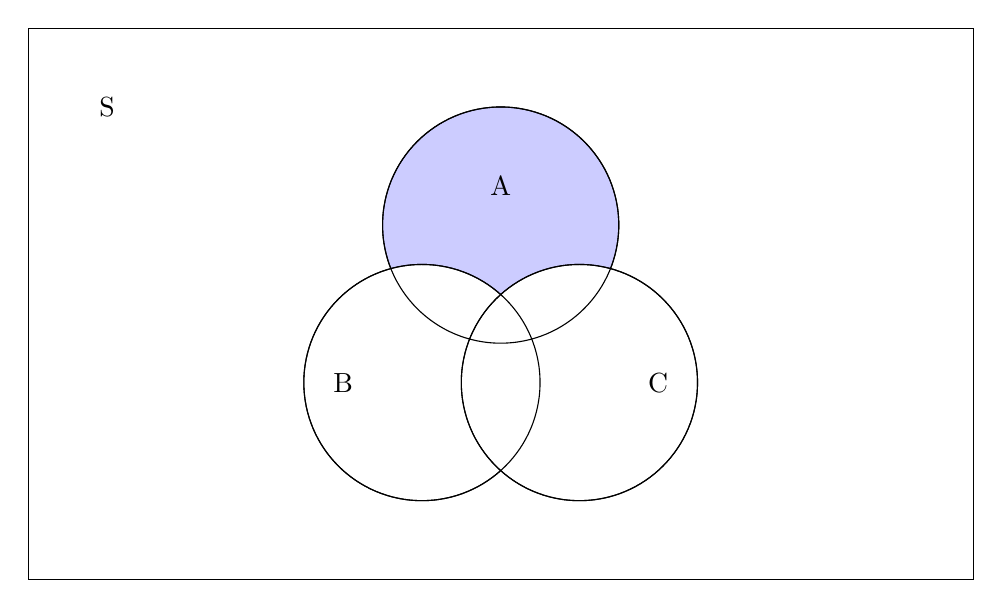
\begin{tikzpicture}
			\draw[fill=black!0] (0,0) rectangle (12,7);
  			\draw[fill=blue!20] (6,4.5) circle (1.5cm); % Circle A
  			\draw[fill=red!0] (5,2.5) circle (1.5cm); % Circle B
  			\draw[fill=green!0] (7,2.5) circle (1.5cm); % Circle C
  			\draw (6,4.5) circle (1.5cm); % Outline of Circle A
  			\draw (5,2.5) circle (1.5cm); % Outline of Circle B
  			\draw (7,2.5) circle (1.5cm); % Outline of Circle C
  			\node at (6,5) {A}; % Label for Circle A
  			\node at (4,2.5) {B}; % Label for Circle B
  			\node at (8,2.5) {C}; % Label for Circle C
  			\draw (0,0) rectangle (12,7); % Rectangle S
  			\node at (1,6) {S}; % Label for Rectangle S
		\end{tikzpicture}
		
		
		\item This is the Venn Diagram where at least one of the events $A$, $B$, or $C$ occurs.

		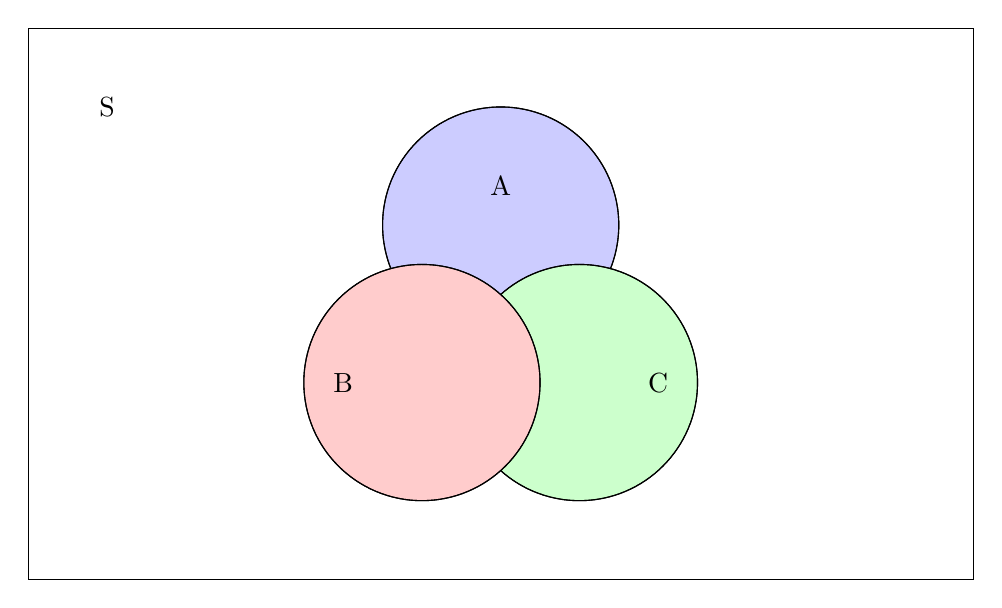
\begin{tikzpicture}
			\draw[fill=black!0] (0,0) rectangle (12,7);
			
  			\draw[fill=blue!20] (6,4.5) circle (1.5cm); % Circle A
  			\draw (6,4.5) circle (1.5cm); % Outline of Circle A
  			
  			\draw[fill=green!20] (7,2.5) circle (1.5cm); % Circle C
  			\draw (7,2.5) circle (1.5cm); % Outline of Circle C
  			
  			\draw[fill=red!20] (5,2.5) circle (1.5cm); % Circle B
  			\draw (5,2.5) circle (1.5cm); % Outline of Circle B
  			
  			\node at (6,5) {A}; % Label for Circle A
  			\node at (4,2.5) {B}; % Label for Circle B
  			\node at (8,2.5) {C}; % Label for Circle C
  			\draw (0,0) rectangle (12,7); % Rectangle S
  			\node at (1,6) {S}; % Label for Rectangle S
		\end{tikzpicture}
		
		\item This is the Venn Diagram where one of $A$ or $C$ occurs, but not $B$.
		
		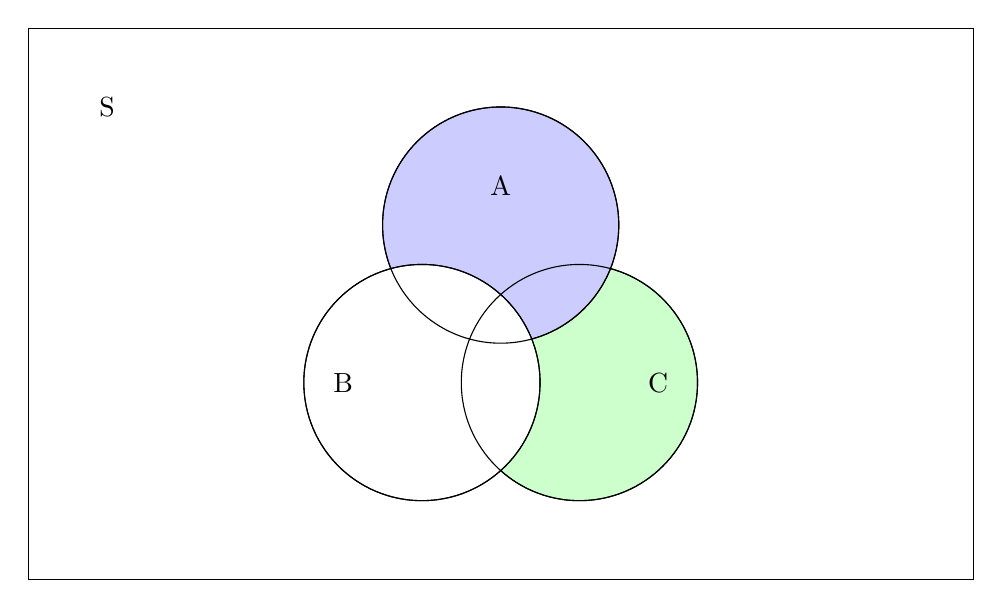
\begin{tikzpicture}
			\draw[fill=black!0] (0,0) rectangle (12,7);
			\draw[fill=green!20] (7,2.5) circle (1.5cm); % Circle C
  			\draw[fill=blue!20] (6,4.5) circle (1.5cm); % Circle A
  			\draw[fill=red!0] (5,2.5) circle (1.5cm); % Circle B
  			\draw (6,4.5) circle (1.5cm); % Outline of Circle A
  			\draw (7,2.5) circle (1.5cm); % Outline of Circle C
  			\draw (5,2.5) circle (1.5cm); % Outline of Circle B  	
  			\node at (6,5) {A}; % Label for Circle A
  			\node at (4,2.5) {B}; % Label for Circle B
  			\node at (8,2.5) {C}; % Label for Circle C
  			\draw (0,0) rectangle (12,7); % Rectangle S
  			\node at (1,6) {S}; % Label for Rectangle S
		\end{tikzpicture}
		
		\item This is the Venn Diagram where at most, two of the events $A$, $B$, or $C$ occurs.
		
		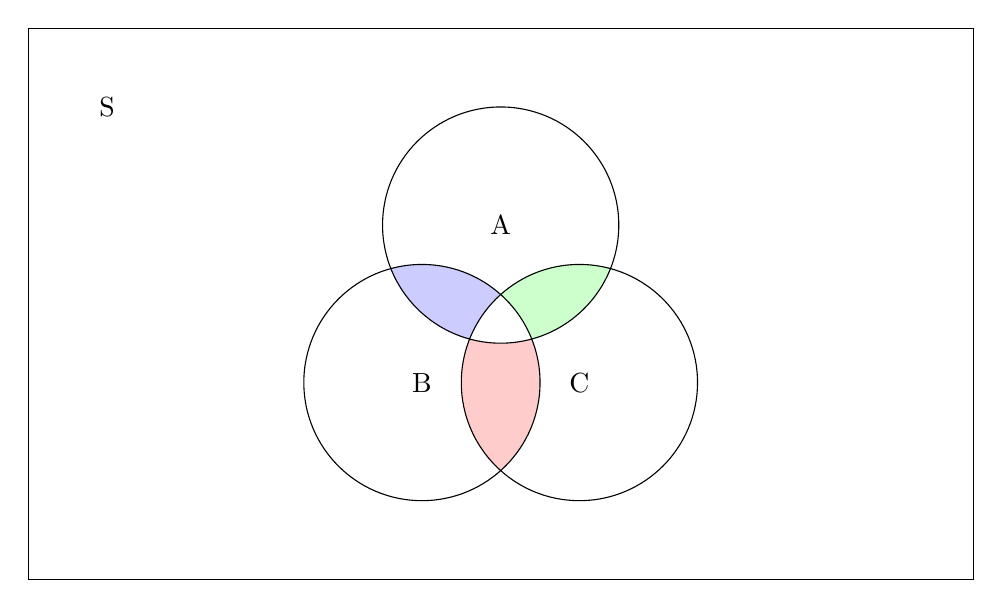
\begin{tikzpicture}
			\draw[fill=black!0] (0,0) rectangle (12,7);
  			\begin{scope} % Scope for transparency
    			\clip (6,4.5) circle (1.5cm); % Circle A
    			\fill[blue!20] (5,2.5) circle (1.5cm); % Circle B
    			\fill[blue!20] (7,2.5) circle (1.5cm); % Circle C
  			\end{scope}
  			\begin{scope} % Scope for transparency
    			\clip (5,2.5) circle (1.5cm); % Circle B
    			\fill[red!20] (7,2.5) circle (1.5cm); % Circle C
  			\end{scope}
  			\begin{scope} % Scope for transparency
    			\clip (7,2.5) circle (1.5cm); % Circle C
    			\fill[green!20] (6,4.5) circle (1.5cm); % Circle A
  			\end{scope}
  			\begin{scope} % Scope for intersection ABC
    			\clip (6,4.5) circle (1.5cm);
    			\clip (5,2.5) circle (1.5cm);
    			\clip (7,2.5) circle (1.5cm);
    			\fill[white] (6,3.5) circle (1.5cm);
  			\end{scope}
  			\draw (6,4.5) circle (1.5cm) node {A}; % Outline of Circle A
  			\draw (5,2.5) circle (1.5cm) node {B}; % Outline of Circle B
  			\draw (7,2.5) circle (1.5cm) node {C}; % Outline of Circle C
  			\draw (0,0) rectangle (12,7); % Rectangle S
  			\node at (1,6) {S}; % Label for Rectangle S
		\end{tikzpicture}
	\end{enumerate}
	
	\item 
	\begin{proof}
	``$A$ and $B$ are independent $\Leftrightarrow$ $A^{c}$ and $B$ are independent."
	
	``$\Rightarrow$": Since $A$ and $B$ are independent, we have:
	$$P(A \cap B) = P(A)P(B) \qquad (\triangle)$$ 
	by Definition 2.18 (independence).
	Now we want to show that:
	$$P(A^{c} \cap B) = P(A^{c})P(B)$$
	We know that:
	$$P(B) = P(A^{c} \cap B) + P(A \cap B) \qquad (\theta)$$ 
	because the probability of $B$, is the same as probability of $A$ and $B$ happening added with probability of $\neg A$ and $B$. We then also learn that:
%	$$P(A^{c} \cap B) = P(B) - P(A \cap B) \qquad (\Theta)$$
	by rearranging $(\delta)$. 
	
	We will now substitute $(\triangle)$ into $(\Theta)$  where we will have
	$$P(A^{c} \cap B) = P(B) - P(A)P(B)$$
	$$P(A^{c} \cap B) = P(B)(1 - P(A)) \qquad (\vert)$$
	and by Theorem 2.19 (Complement Rule), we learn that
	$$(1 - P(A)) = P(A^{c})$$
	then this equation,
	$$P(A^{c} \cap B) = P(A^{c})P(B)$$
	is identical to $(\vert)$. Hence we have proven that 
	
	$$A \text{ and } B \text{ are independent } \Rightarrow A^{c} \text{ and } B \text{ are independent.}$$ 

	``$\Leftarrow$": Now, since $A^c$ and $B$ are independent, we have:
	$$P(A^c \cap B) = P(A^c)P(B) \qquad (\phi)$$ 
	by Definition 2.18 (independence). This proof is trivial as it follows the same structure as the last one I did.
	Now we want to show that:
	$$P(A \cap B) = P(A)P(B)$$
	We know that:
	$$P(B) = P(A^{c} \cap B) + P(A \cap B) \qquad (\gamma)$$ 
	because the probability of $B$, is the same as probability of $A$ and $B$ happening added with probability of $\neg A$ and $B$. We then also learn that:
	$$P(A \cap B) = P(B) - P(A^c \cap B) \qquad (\Gamma)$$
	by rearranging $(\gamma)$. 
	
	We will now substitute $(\phi)$ into $(\gamma)$  where we will have
	$$P(A \cap B) = P(B) - P(A^c)P(B)$$
	$$P(A \cap B) = P(B)(1 - P(A^c)) \qquad (\psi)$$
	and by Theorem 2.19 (Complement Rule), we learn that
	$$(1 - P(A^c)) = P(A)$$
	then this equation,
	$$P(A \cap B) = P(A)P(B)$$
	is identical to $(\psi)$. Hence we have proven that 
	$$A^{c} \text{ and } B \text{ are independent } \Rightarrow A \text{ and } B \text{ are independent.} $$ 
	Therefore, We have proven that $A$ and $B$ are independent $\Leftrightarrow$ $A^c$ and $B$ are independent. \qedhere 
	\end{proof}
	
	\item Let $S$ be the event that the silver coin is found and let $C$ be the event that a cabinet was selected.

	We know that
	$$P(C_A) = P(C_B) = \frac{1}{2}$$
	because both drawers in cabinet A ($C_A$) contains the silver coin, we have 
	$$P(S|C_A) = \frac{1}{2} + \frac{1}{2} = 1$$
	and because only one of the silver coin is in cabinet B ($C_B$), we have
	$$P(S|C_B) = \frac{1}{2}$$
	Using Theorem 2.20 (Rule of Probability), then we learn that 
	$$P(S) = P(S|C_A)P(C_A) + P(S|C_B)P(C_B)$$
	$$= (1 \times \frac{1}{2}) + (\frac{1}{2} \times \frac{1}{2})$$
	$$= \frac{3}{4}$$
	and using Theorem 2.21 (Bayes' Theorem), we can conclude that
	$$P(C|S) = \frac{P(S|C)P(C)}{P(S)} = \frac{1 \times \frac{1}{2}}{\frac{3}{4}} = \frac{2}{3}$$
	
	End of Assignment 1.
	
	
	
	
	
	
	
\end{enumerate}

\end{document}
